% Options for packages loaded elsewhere
\PassOptionsToPackage{unicode}{hyperref}
\PassOptionsToPackage{hyphens}{url}
%
\documentclass[
  ignorenonframetext,
]{beamer}
\usepackage{pgfpages}
\setbeamertemplate{caption}[numbered]
\setbeamertemplate{caption label separator}{: }
\setbeamercolor{caption name}{fg=normal text.fg}
\beamertemplatenavigationsymbolsempty
% Prevent slide breaks in the middle of a paragraph
\widowpenalties 1 10000
\raggedbottom
\setbeamertemplate{part page}{
  \centering
  \begin{beamercolorbox}[sep=16pt,center]{part title}
    \usebeamerfont{part title}\insertpart\par
  \end{beamercolorbox}
}
\setbeamertemplate{section page}{
  \centering
  \begin{beamercolorbox}[sep=12pt,center]{part title}
    \usebeamerfont{section title}\insertsection\par
  \end{beamercolorbox}
}
\setbeamertemplate{subsection page}{
  \centering
  \begin{beamercolorbox}[sep=8pt,center]{part title}
    \usebeamerfont{subsection title}\insertsubsection\par
  \end{beamercolorbox}
}
\AtBeginPart{
  \frame{\partpage}
}
\AtBeginSection{
  \ifbibliography
  \else
    \frame{\sectionpage}
  \fi
}
\AtBeginSubsection{
  \frame{\subsectionpage}
}
\usepackage{amsmath,amssymb}
\usepackage{lmodern}
\usepackage{iftex}
\ifPDFTeX
  \usepackage[T1]{fontenc}
  \usepackage[utf8]{inputenc}
  \usepackage{textcomp} % provide euro and other symbols
\else % if luatex or xetex
  \usepackage{unicode-math}
  \defaultfontfeatures{Scale=MatchLowercase}
  \defaultfontfeatures[\rmfamily]{Ligatures=TeX,Scale=1}
\fi
\usecolortheme{beaver}
% Use upquote if available, for straight quotes in verbatim environments
\IfFileExists{upquote.sty}{\usepackage{upquote}}{}
\IfFileExists{microtype.sty}{% use microtype if available
  \usepackage[]{microtype}
  \UseMicrotypeSet[protrusion]{basicmath} % disable protrusion for tt fonts
}{}
\makeatletter
\@ifundefined{KOMAClassName}{% if non-KOMA class
  \IfFileExists{parskip.sty}{%
    \usepackage{parskip}
  }{% else
    \setlength{\parindent}{0pt}
    \setlength{\parskip}{6pt plus 2pt minus 1pt}}
}{% if KOMA class
  \KOMAoptions{parskip=half}}
\makeatother
\usepackage{xcolor}
\newif\ifbibliography
\setlength{\emergencystretch}{3em} % prevent overfull lines
\providecommand{\tightlist}{%
  \setlength{\itemsep}{0pt}\setlength{\parskip}{0pt}}
\setcounter{secnumdepth}{-\maxdimen} % remove section numbering
\iffalse
https://tex.stackexchange.com/questions/392324/how-to-exclude-total-slide-number-from-beamer-slide
\fi
\setbeamertemplate{navigation symbols}{} 
\setbeamertemplate{footline}{\quad\hfill\insertframenumber\strut\quad}
\usefonttheme[onlymath]{serif}
\setbeamertemplate{itemize items}[circle]
\author[John Koo]{John Koo}
\usepackage{setspace}
\usepackage{float}
\usepackage{mathtools}
\usepackage{natbib}
\usepackage[linesnumbered,ruled,vlined]{algorithm2e}
\setcitestyle{numbers,square,comma}
\usepackage{verbatim}
\usepackage{amsthm}
\usepackage{comment}
\usepackage{graphicx}
\setbeamertemplate{itemize items}[circle]
\ifLuaTeX
  \usepackage{selnolig}  % disable illegal ligatures
\fi
\IfFileExists{bookmark.sty}{\usepackage{bookmark}}{\usepackage{hyperref}}
\IfFileExists{xurl.sty}{\usepackage{xurl}}{} % add URL line breaks if available
\urlstyle{same} % disable monospaced font for URLs
\hypersetup{
  hidelinks,
  pdfcreator={LaTeX via pandoc}}

\author{}
\date{\vspace{-2.5em}}

\begin{document}

\begin{frame}[plain]{}
\protect\hypertarget{section}{}
\center

\LARGE

\textcolor{darkred}{Manifold Clustering in the Setting of Generalized Random Dot Product Graphs}

\normalsize

SDSS Lightning Presentation

May 2023

\begin{columns}[T]
\begin{column}{0.33\textwidth}
\begin{center}\includegraphics[width=67px]{john-koo} \end{center}

John Koo,\\
Postdoctoral Fellow,\\
Indiana University
\end{column}

\begin{column}{0.33\textwidth}
\begin{center}\includegraphics[width=67px]{minh-tang} \end{center}

Minh Tang,\\
Assistant Professor,\\
NC State University
\end{column}

\begin{column}{0.33\textwidth}
\begin{center}\includegraphics[width=67px]{michael-trosset} \end{center}

Michael W. Trosset,\\
Professor of Statistics,\\
Indiana University
\end{column}
\end{columns}
\end{frame}

\begin{frame}{Community Detection for Networks}
\protect\hypertarget{community-detection-for-networks}{}
\newcommand{\diag}{\text{diag}}
\newcommand{\tr}{\text{Tr}}
\newcommand{\blockdiag}{\text{blockdiag}}
\newcommand{\indep}{\stackrel{\text{ind}}{\sim}}
\newcommand{\iid}{\stackrel{\text{iid}}{\sim}}
\newcommand{\Bernoulli}{\text{Bernoulli}}
\newcommand{\Betadist}{\text{Beta}}
\newcommand{\BG}{\text{BernoulliGraph}}
\newcommand{\Categorical}{\text{Categorical}}
\newcommand{\Uniform}{\text{Uniform}}
\newcommand{\RDPG}{\text{RDPG}}
\newcommand{\GRDPG}{\text{GRDPG}}
\newcommand{\PABM}{\text{PABM}}

\begin{center}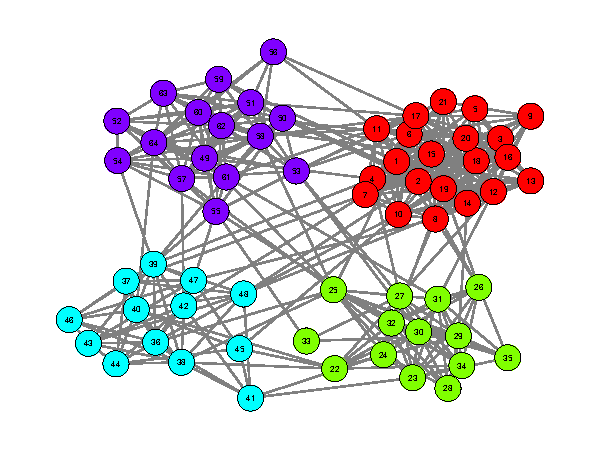
\includegraphics[width=0.5\linewidth]{slides_files/figure-beamer/unnamed-chunk-4-1} \end{center}

\begin{center}

How might we cluster the nodes of a network?

\end{center}
\end{frame}

\begin{frame}{Connecting Block Models to the GRDPG}
\protect\hypertarget{connecting-block-models-to-the-grdpg}{}
\begin{columns}[T]
\begin{column}{0.67\textwidth}
\begin{center}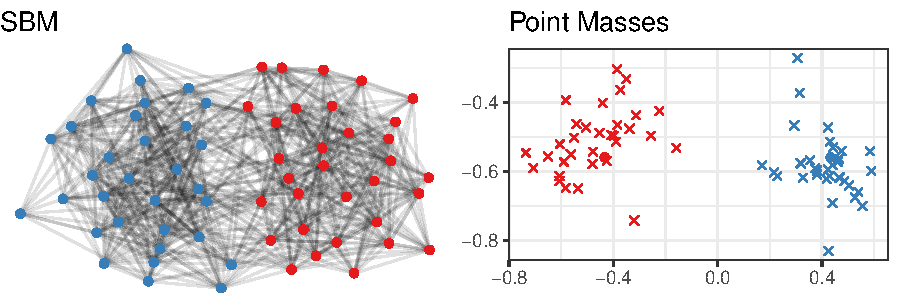
\includegraphics[width=1\linewidth]{slides_files/figure-beamer/unnamed-chunk-5-1} \end{center}

\begin{center}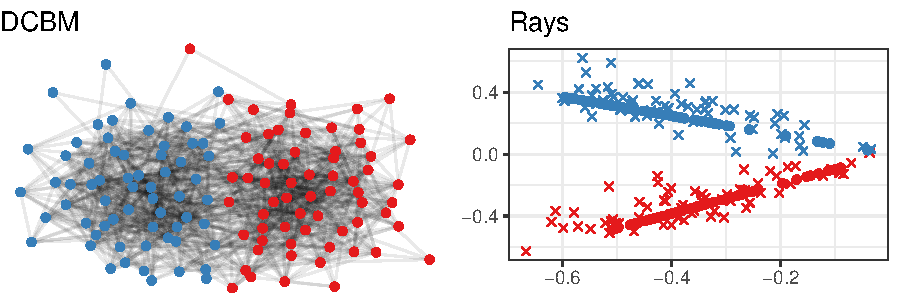
\includegraphics[width=1\linewidth]{slides_files/figure-beamer/unnamed-chunk-6-1} \end{center}

\begin{center}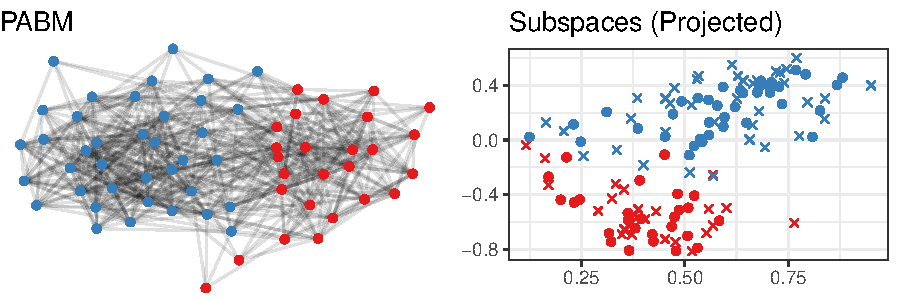
\includegraphics[width=1\linewidth]{slides_files/figure-beamer/unnamed-chunk-7-1} \end{center}
\end{column}

\begin{column}{0.33\textwidth}
~

~

\begin{itemize}
\tightlist
\item
  K-means clustering
\item
  Gaussian mixture models
\end{itemize}

~

\begin{itemize}
\tightlist
\item
  K-means with cosine similarity
\item
  GMM on angles
\end{itemize}

~

~

~

\begin{itemize}
\tightlist
\item
  Orthogonal Spectral Clustering
\item
  Sparse Subspace Clustering
\end{itemize}
\end{column}
\end{columns}
\end{frame}

\begin{frame}{Nonlinear Communty Structure}
\protect\hypertarget{nonlinear-communty-structure}{}
\begin{center}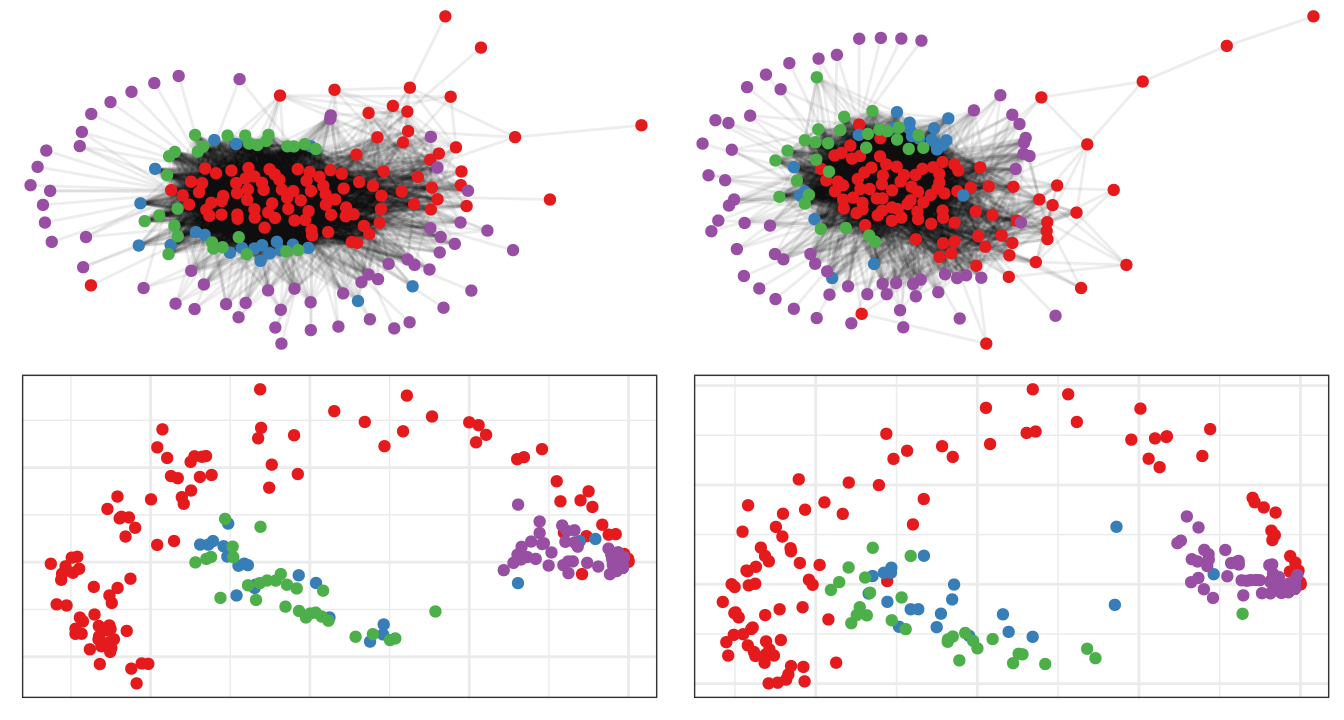
\includegraphics[width=1\linewidth]{slides_files/figure-beamer/mbconnectome-ase-1} \end{center}
\end{frame}

\begin{frame}{Manifold Block Model}
\protect\hypertarget{manifold-block-model}{}
Let \(p, q \geq 0\), \(d = p + q \geq 1\), \(1 \leq r < d\),
\(K \geq 2\), and \(n > K\) be integers. Define manifolds
\(\mathcal{M}_1, ..., \mathcal{M}_K \in \mathcal{X}\) for
\(\mathcal{X} = \{x, y \in \mathbb{R}^d : x^\top I_{p,q} y \in [0, 1]\}\)
each by continuous function \(g_k : [0, 1]^r \to \mathcal{X}\). Define
probability distribution \(F\) with support \([0, 1]^r\). Then the
following mixture model is a \emph{manifold block model}:

\begin{enumerate}
\item Draw labels $z_1, ..., z_n \stackrel{\text{iid}}{\sim}\text{Categorical}(\alpha_1, ..., \alpha_K)$.
\item Draw latent vectors by first taking $t_1,..., t_n \stackrel{\text{iid}}{\sim}F$ and then computing each $x_i = g_{z_i}(t_i)$. 
\item Compile the latent vectors into data matrix $X = [ x_1 \mid \cdots \mid x_n ]^\top$ and define the adjacency matrix as $A \sim \text{GRDPG}_{p,q}(X)$. 
\end{enumerate}
\end{frame}

\begin{frame}{Manifold Block Model}
\protect\hypertarget{manifold-block-model-1}{}
\begin{enumerate}
\tightlist
\item
  \(z_1, ..., z_n \stackrel{\text{iid}}{\sim}\text{Categorical}(1/2, 1/2)\)
\item
  \(t_1, ..., t_n \stackrel{\text{iid}}{\sim}\text{Uniform}(0, 1)\)
\item
  \(x_i = g_{z_i}(t_i)\)

  \begin{itemize}
  \tightlist
  \item
    \(g_1(t) = [t^2, 2 t (1-t)]^\top\)
  \item
    \(g_2(t) = [2 t (1-t), (1-t)^2]^\top\)
  \end{itemize}
\item
  \(A \sim \text{GRDPG}_{2, 0}(X)\)
\end{enumerate}

\begin{figure}

{\centering \includegraphics[width=1\linewidth]{slides_files/figure-beamer/intersect-curves-example-1} 

}

\caption{Latent vectors on intersecting curves (left), along with an RDPG drawn from this configuration (center) and its ASE (right).}\label{intersect-curves-example}
\end{figure}
\end{frame}

\begin{frame}{\(K\)-Curves Clustering}
\protect\hypertarget{k-curves-clustering}{}
\begin{algorithm}[H]
\label{alg:kcurves}
\scriptsize
\DontPrintSemicolon
\SetAlgoLined
\KwData{Adjacency matrix $A$, number of communities $K$, embedding dimensions $p$, $q$, stopping criterion $\epsilon$}
\KwResult{Community assignments $1, ..., K$, curves $g_1, ..., g_K$}
Compute $X$, the ASE of $A$ using the $p$ most positive and $q$ most negative eigenvalues and their corresponding eigenvectors.\;
Initialize community labels $z_1, ..., z_n$.\;
\Repeat {the change in $\sum_k \sum_{i \in C_k} \|x_i - g_k(t_i)\|^2$ is less than $\epsilon$} {
\For {$k = 1, ..., K$} {
Define $X_k$ as the rows of $X$ for which $z_i = k$.\;
Fit curve $g_k$ and positions $t_{k_i}$ to $X_k$ by minimizing $\sum_{k_i} \|x_{k_i} - g_k(t_{k_i})\|^2$.\;
}
\For {$k = 1, ..., K$} {
Assign $z_i \leftarrow \arg\min_\ell \|x_i - g_\ell(t_i)\|^2$.\;
}
}
\caption{$K$-curves clustering.}
\end{algorithm}
\end{frame}

\begin{frame}{Example}
\protect\hypertarget{example}{}
\begin{center}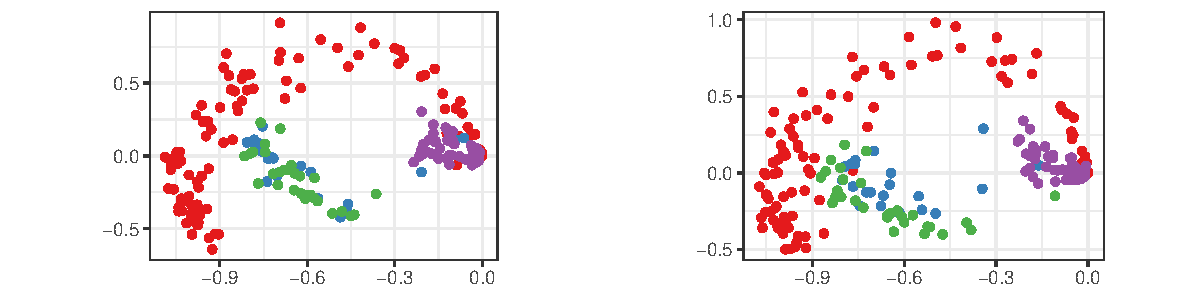
\includegraphics[width=1\linewidth]{slides_files/figure-beamer/mbconnectome-ase-2-1} \end{center}

\begin{center}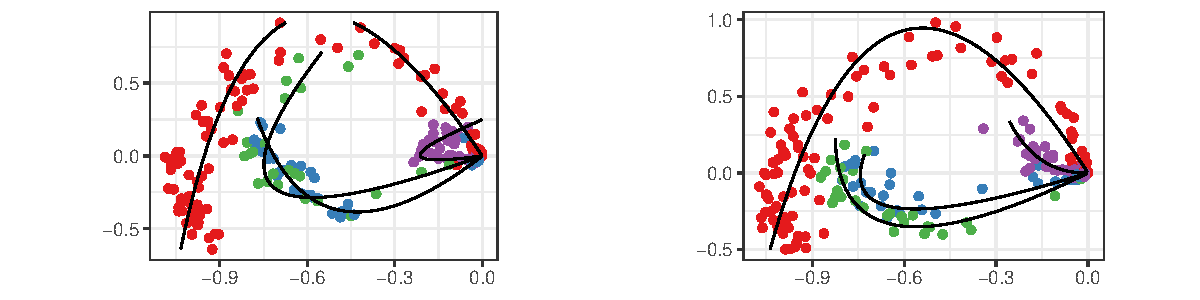
\includegraphics[width=1\linewidth]{slides_files/figure-beamer/mbconnectome-kcurves-1} \end{center}
\end{frame}

\begin{frame}{Asymptotic Results}
\protect\hypertarget{asymptotic-results}{}
\textbf{Theorem}. Let an MBM be such that the manifolds are described by
functions \(g_1(t), ..., g_K(t)\) which are polynomial curves of order
\(R\). Define the loss of \(K\)-curves clustering as:

\[L(\hat{z}_1, ..., \hat{z}_n, \hat{g}_1, ..., \hat{g}_K; A) = \sum_k \sum_{i : \hat{z}_i = k} \|\hat{x}_{i} - \hat{g}_k(t_{i})\|^2,\]

where \(\hat{x}_i\) are the embedding vectors of \(A\). Suppose that for
each community \(k\), we have labels for at least \(R + 1\) vertices.
Then as \(n \to \infty\), \(K\)-curves clustering outputs estimates such
that

\[L(\hat{z}_1, ..., \hat{z}_n, \hat{g}_1, ..., \hat{g}_K; A) \stackrel{p}{\to} 0.\]
\end{frame}

\begin{frame}{Simulation}
\protect\hypertarget{simulation}{}
\begin{center}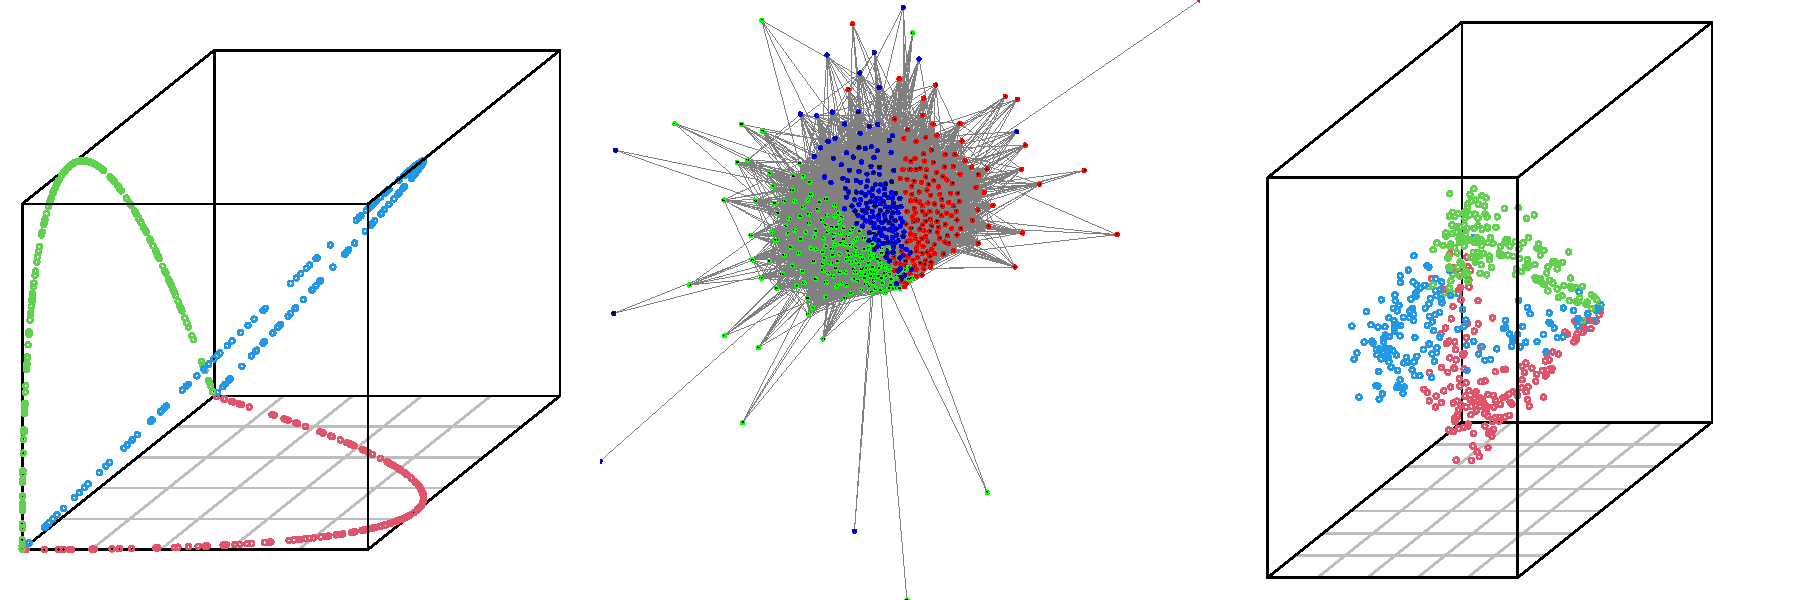
\includegraphics[width=1\linewidth]{slides_files/figure-beamer/three-curves-1} \end{center}

\begin{center}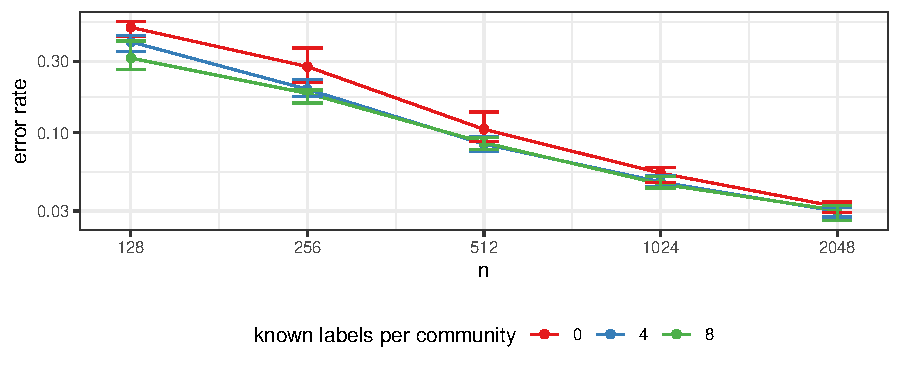
\includegraphics[width=1\linewidth]{slides_files/figure-beamer/sim-curves-3-1} \end{center}
\end{frame}

\begin{frame}{Thank you!}
\protect\hypertarget{thank-you}{}
Code and drafts available at
\url{https://github.com/johneverettkoo/manifold-block-models}
\end{frame}

\end{document}
